\chapter{\ifproject%
\ifcpe โครงสร้างและขั้นตอนการทำงาน\else Project Structure and Methodology\fi
\else%
\ifcpe โครงสร้างของโครงงาน\else Project Structure\fi
\fi
}

ในบทนี้จะกล่าวถึงหลักการ และการออกแบบระบบ

\makeatletter

% \renewcommand\section{\@startsection {section}{1}{\z@}%
%                                    {13.5ex \@plus -1ex \@minus -.2ex}%
%                                    {2.3ex \@plus.2ex}%
%                                    {\normalfont\large\bfseries}}

\makeatother
%\vspace{2ex}
% \titleformat{\section}{\normalfont\bfseries}{\thesection}{1em}{}
% \titlespacing*{\section}{0pt}{10ex}{0pt}



\section{โครงสร้างของระบบ}



\subsection{Database Design}

ประเภทของฐานข้อมูลที่ใช้เป็นแบบ NOSQL
รูปที่~\ref{fig:DatabaseDiagram} แสดงองค์ประกอบต่างๆ ของฐานข้อมูล ซึ่งมีรายละเอียดดังนี้
%
  \begin{itemize}
    \item childs เก็บข้อมูลที่เกี่ยวข้องกับเด็กทั้งหมด อาทิเช่น เก็บวันที่สมัคร วันที่เข้าเรียน ชื่อ ชื่อเล่น วันเดือนปีเกิด และ อื่นๆ มีจะมีอยู่ 2 attributes ที่ใช้เชื่อมความสัมพันธ์กับ Collection อื่น ก็คือ ตัว \_id และ child\_id 
    โดยที่ \_id จะมีการเชื่อมกับ payment , gadgets , healths , stock , rooms
    ส่วน child\_id จะมีการเชื่อมกับ custodian , mother , address , attendances ,father 
    ในส่วนของการเชื่อมความสัมพันธ์นี้ทำ   เพื่อให้เวลาจะมีการเรียกใช้ข้อมูลของเด็กใน ส่วนของข้อมูลอื่น เช่น การเช็คชื่อ การชำระเงินค่าเรียน การเช็คของ    การทำเช่นนี้จะช่วยให้เรียกข้อมูลเด็กมาใช้ได้ง่ายขึ้น
    \item father เก็บข้อมูลส่วนตัวของพ่อเด็ก อาทิเช่น ชื่อ ทำอาชีพอะไร อีเมล เบอร์โทร เป็นต้น
    \item mother เก็บข้อมูลส่วนตัวของแม่เด็ก อาทิเช่น ชื่อ ทำอาชีพอะไร อีเมล เบอร์โทร เป็นต้น
    \item custodian เก็บข้อมูลส่วนตัวของผู้ปกครองเด็ก อาทิเช่น ชื่อ ทำอาชีพอะไร อีเมล เบอร์โทร มีความสัมพันธ์อะไรกับเด็ก เป็นต้น
    \item address เก็บข้อมูลที่อยู่ของเด็ก เช่น บ้านเลขที่ ถนน ตำบล อำเภอ จังหวัด รหัสไปรษณีย์ 
    \item users เก็บ Username Password สำหรับเข้าสู่ ระบบจัดการ Nursery 
    \item buttonchecks เก็บข้อมูลสำหรับใช้เช็คว่าวันนี้มีการเช็คชื่อไปยัง มีการเก็บ วัน ห้อง ประเภท ( เช็คชื่อ ,เช็คของ ,เช็คสุขภาพ )
    \item date\_for\_checks เก็บวันที่ใช้ในการเช็คชื่อย้อนหลัง
    \item rooms เก็บข้อมูลการเรียนของเด็กในห้องต่างๆ มีการเก็บ ข้อมูลเด็ก ห้อง วันที่เข้าเรียน สถานะว่ายังอยู่ในห้องนี้รึเปล่า
    \item attendances เก็บข้อมูลการเช็คชื่อทั้งหมด มีการเก็บ child\_id วันที่เช็ค สถานะว่ามาหรือไม่มา
    \item gadgets เก็บข้อมูลการเช็คอุปกรณ์ของเด็กทั้งหมด มีการเก็บ ข้อมูลเด็ก วัน ลิสต์ของที่ต้องเช็ค ก็จะมีสถานะว่าเอามากับไม่เอา
    \item healths เก็บข้อมูลการเช็คสุขภาพของเด็กทั้งหมด มีการเก็บ ข้อมูลเด็ก วัน ลิสต์สุขภาพที่ต้องเช็ค ก็จะมีสถานะว่าใช่หรือไม่
    \item stock เก็บข้อมูลของใช้ทั้งหมดของเด็กใน Nursery มีการเก็บ ข้อมูลเด็ก วันที่มีการเพิ่มหรือแก้ไขข้อมูล ชื่อของ รายละเอียดของ
    \item payment เก็บข้อมูลประวัติการโอนเงินค่าเล่าเรียนของผู้ปกครองเด็ก มีการเก็บ ข้อมูลเด็ก วันที่ส่งสลิปโอนเงิน ค่าเล่าเรียนหรือจำนวนเงินที่ชำระ รูปสลิปใบเสร็จ 
  \end{itemize}
%
% \afterpage{
  \begin{landscape}
    \begin{figure}
      \begin{center}
      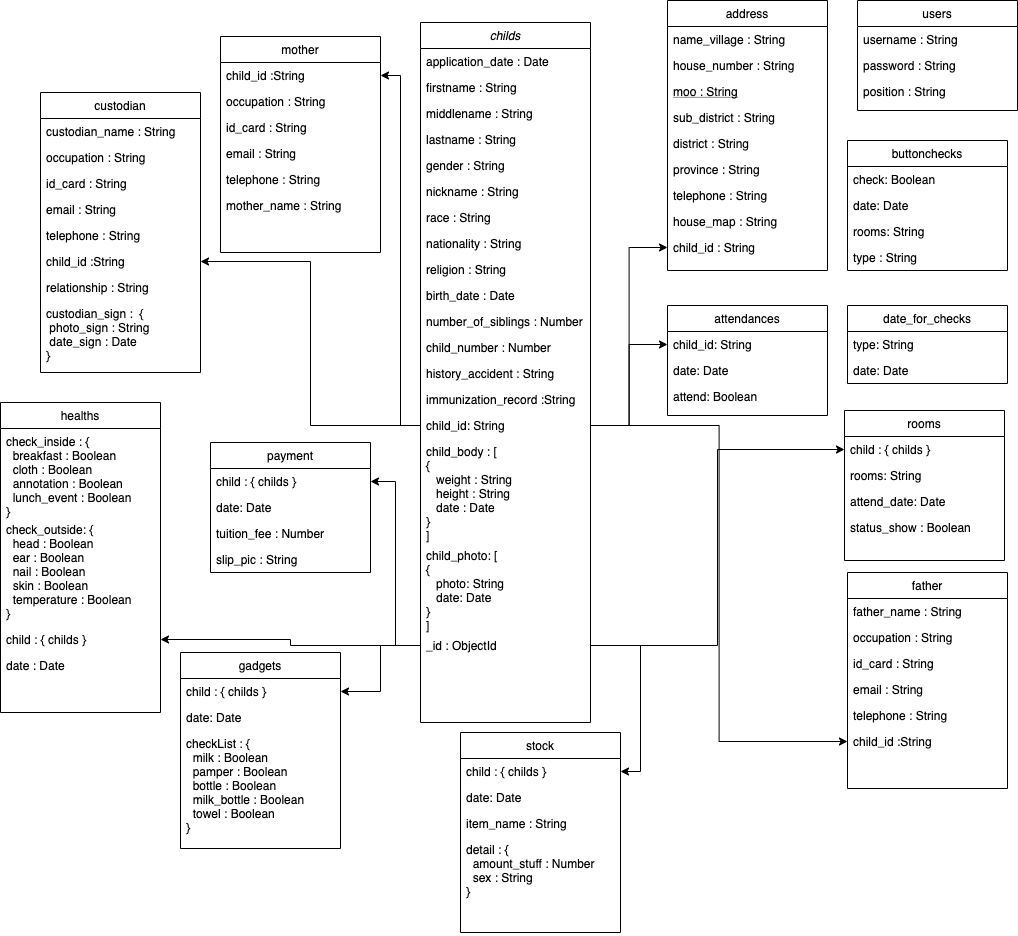
\includegraphics[height=0.9\textheight]{images/databaseDiagram.png}
      \end{center}
    \caption{แผนภาพแสดงรายละเอียดฐานข้อมูลของระบบ}
    \label{fig:DatabaseDiagram}
  \end{figure}
\end{landscape}
% }

\subsection{XD Design}

\begin{figure}
  \begin{center}
  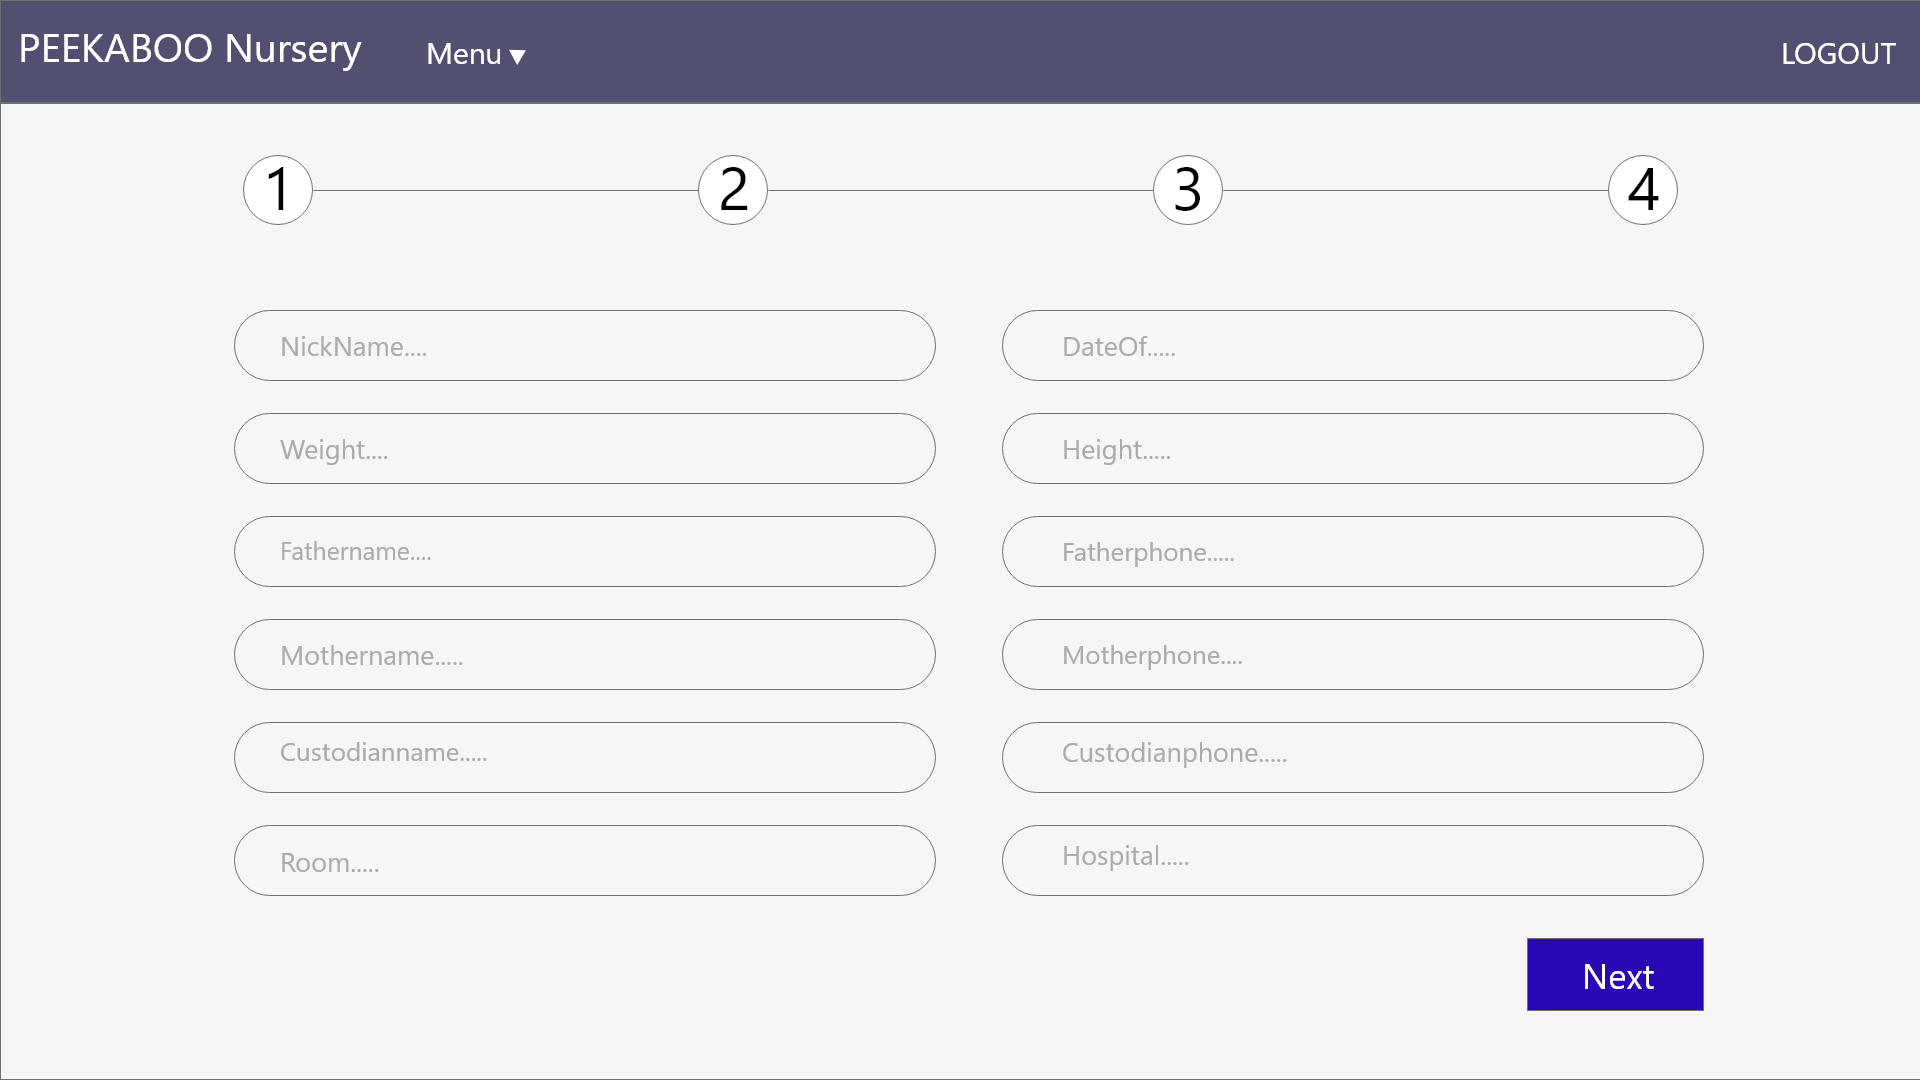
\includegraphics[width=\linewidth]{images/registerPage.png}
  \end{center}
  \caption[Poem]{Register Page}
  \label{fig:register}
  \end{figure}

\begin{figure}
  \begin{center}
  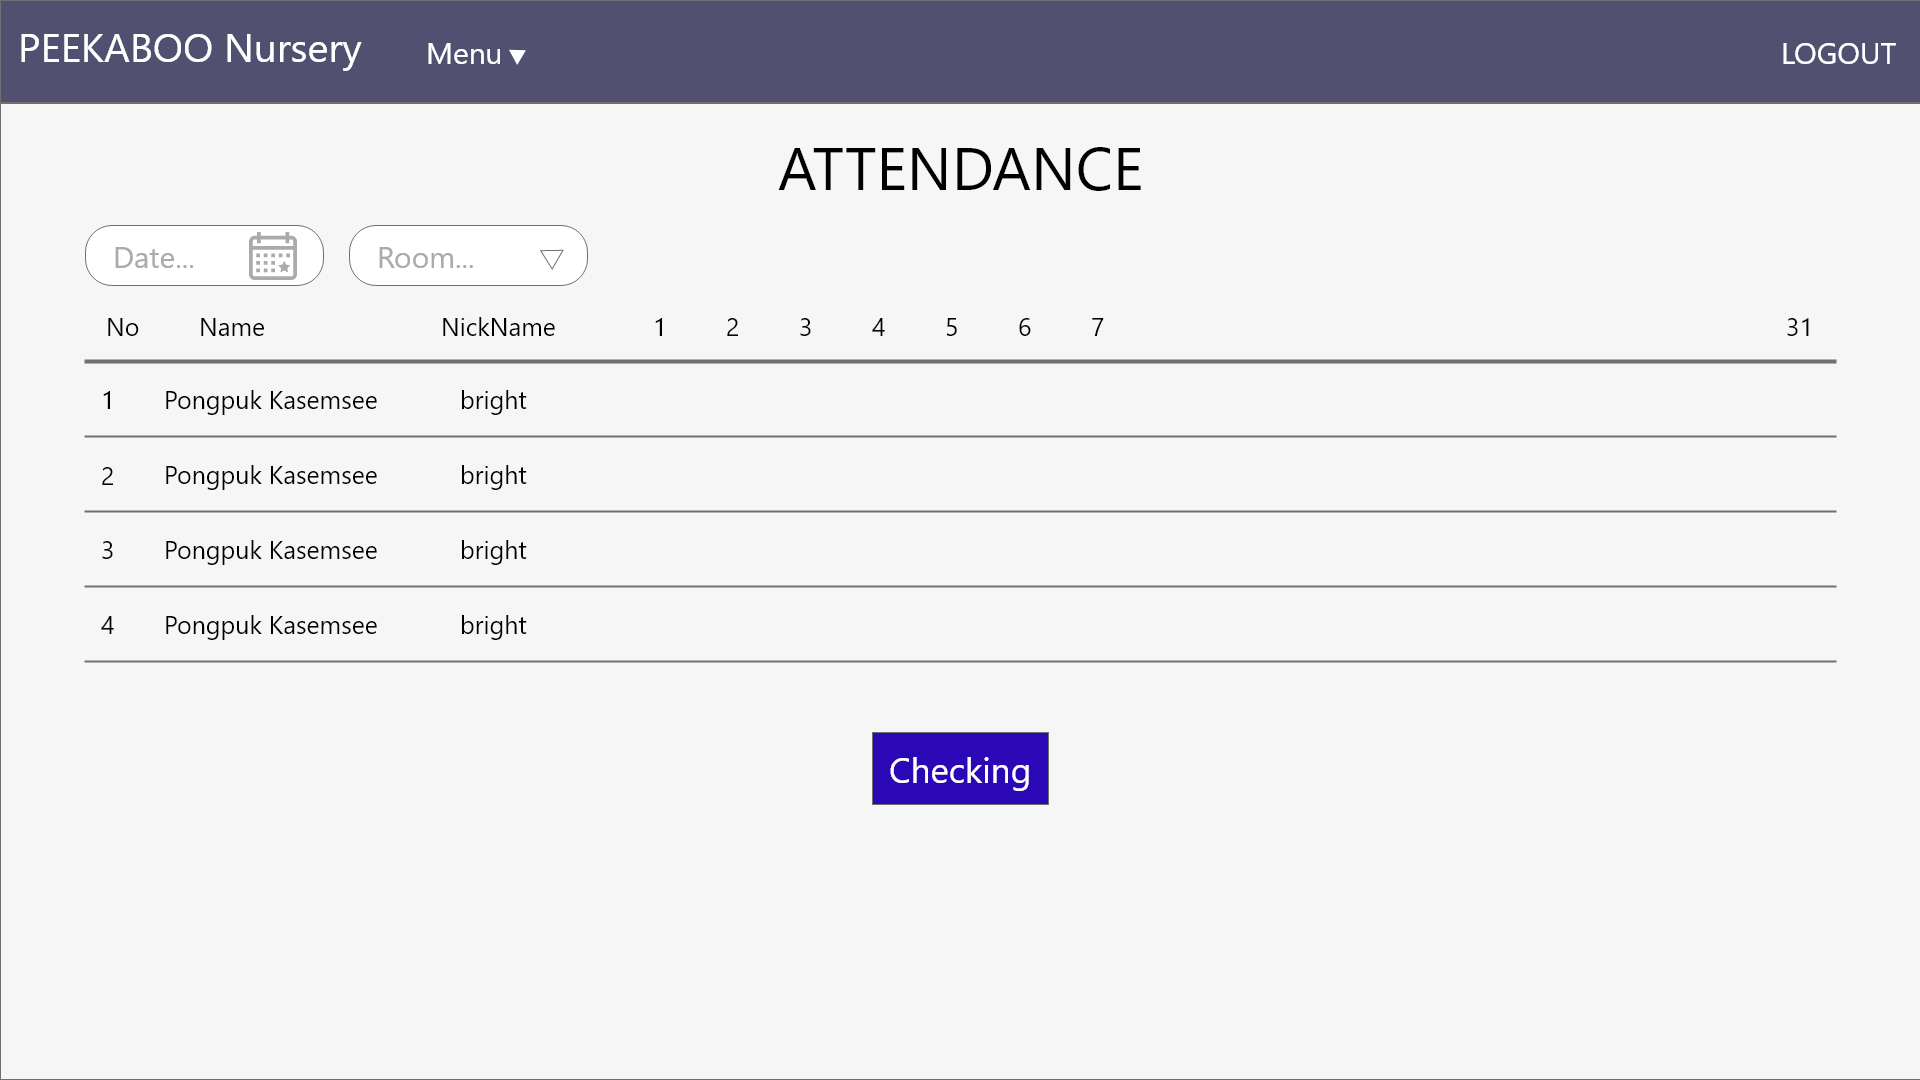
\includegraphics[width=\linewidth]{images/AttendancePage.png}
  \end{center}
  \caption[Poem]{Attendance Page}
  \label{fig:Attendance}
  \end{figure}

\begin{figure}
  \begin{center}
  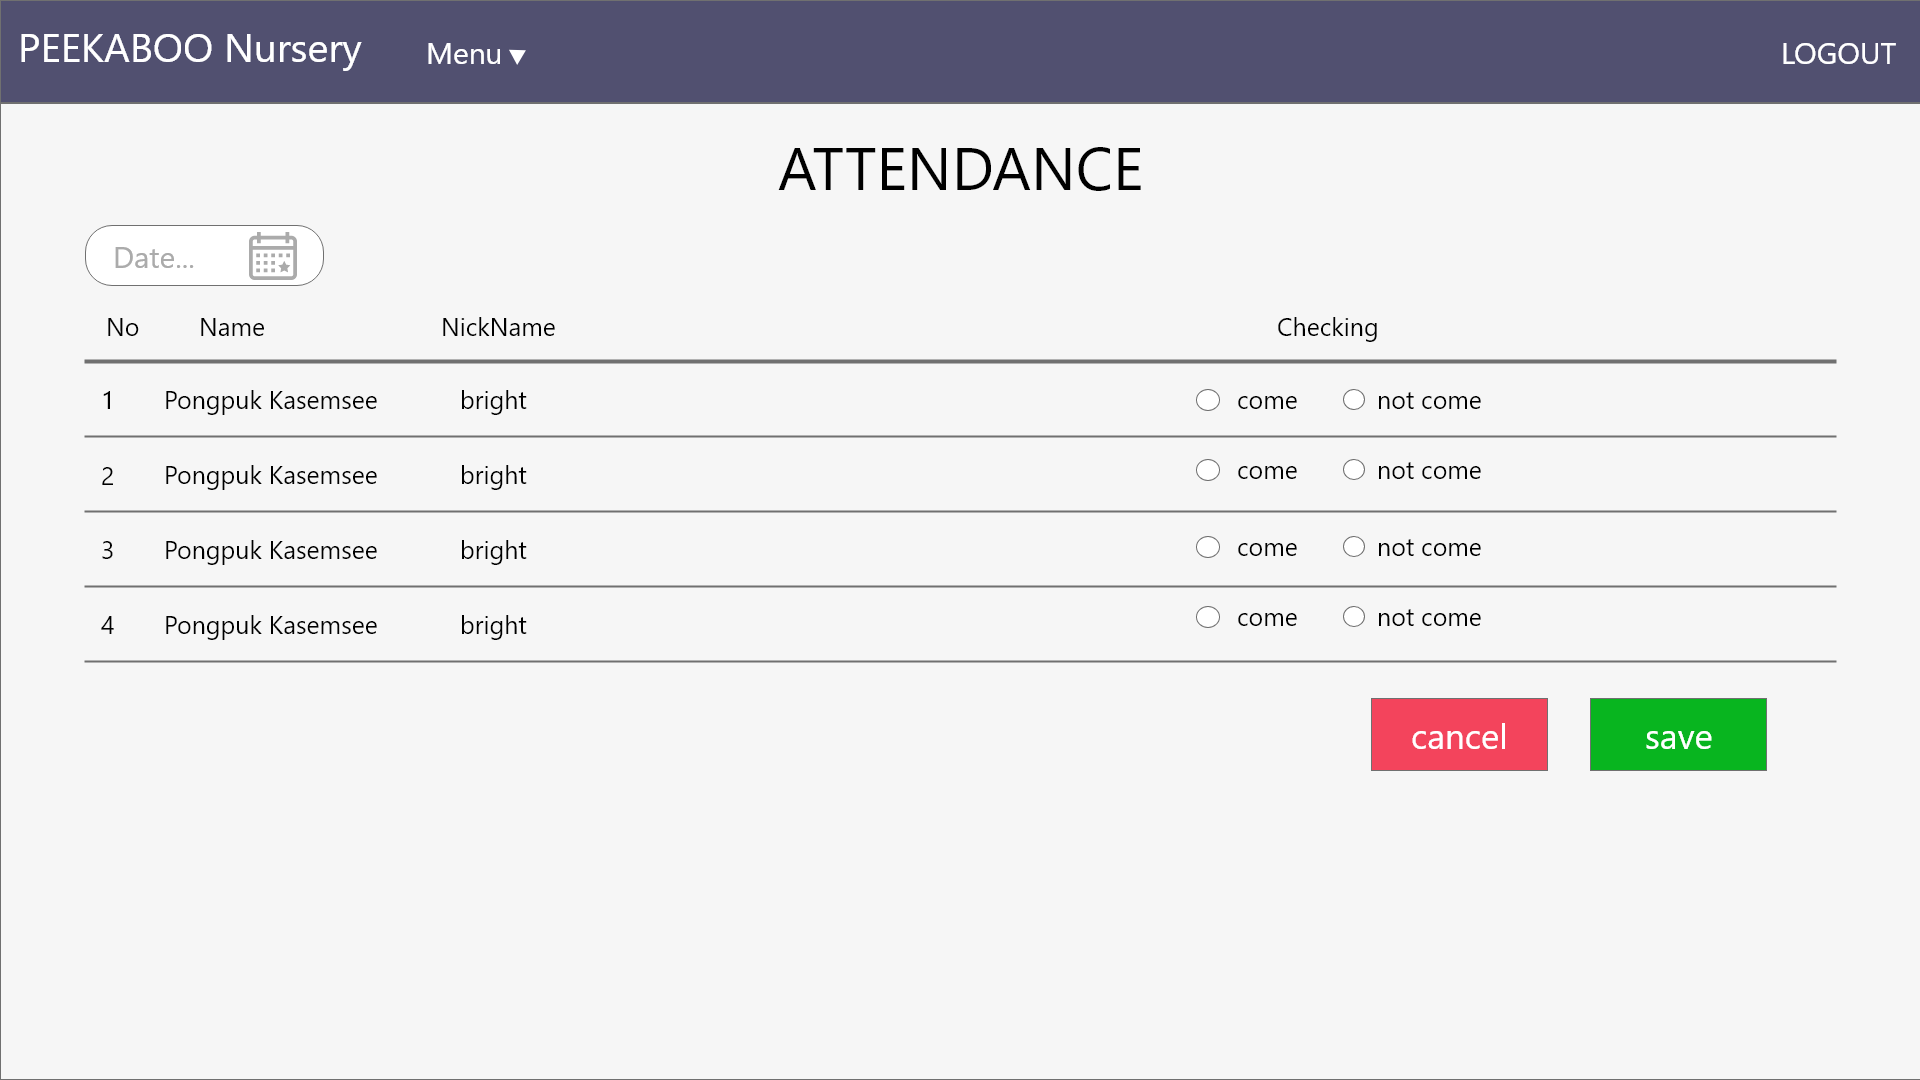
\includegraphics[width=\linewidth]{images/AttendancePageChecking.png}
  \end{center}
  \caption[Poem]{Attendance Checking Page}
  \label{fig:CheckAttendance}
  \end{figure}

\begin{figure}
  \begin{center}
  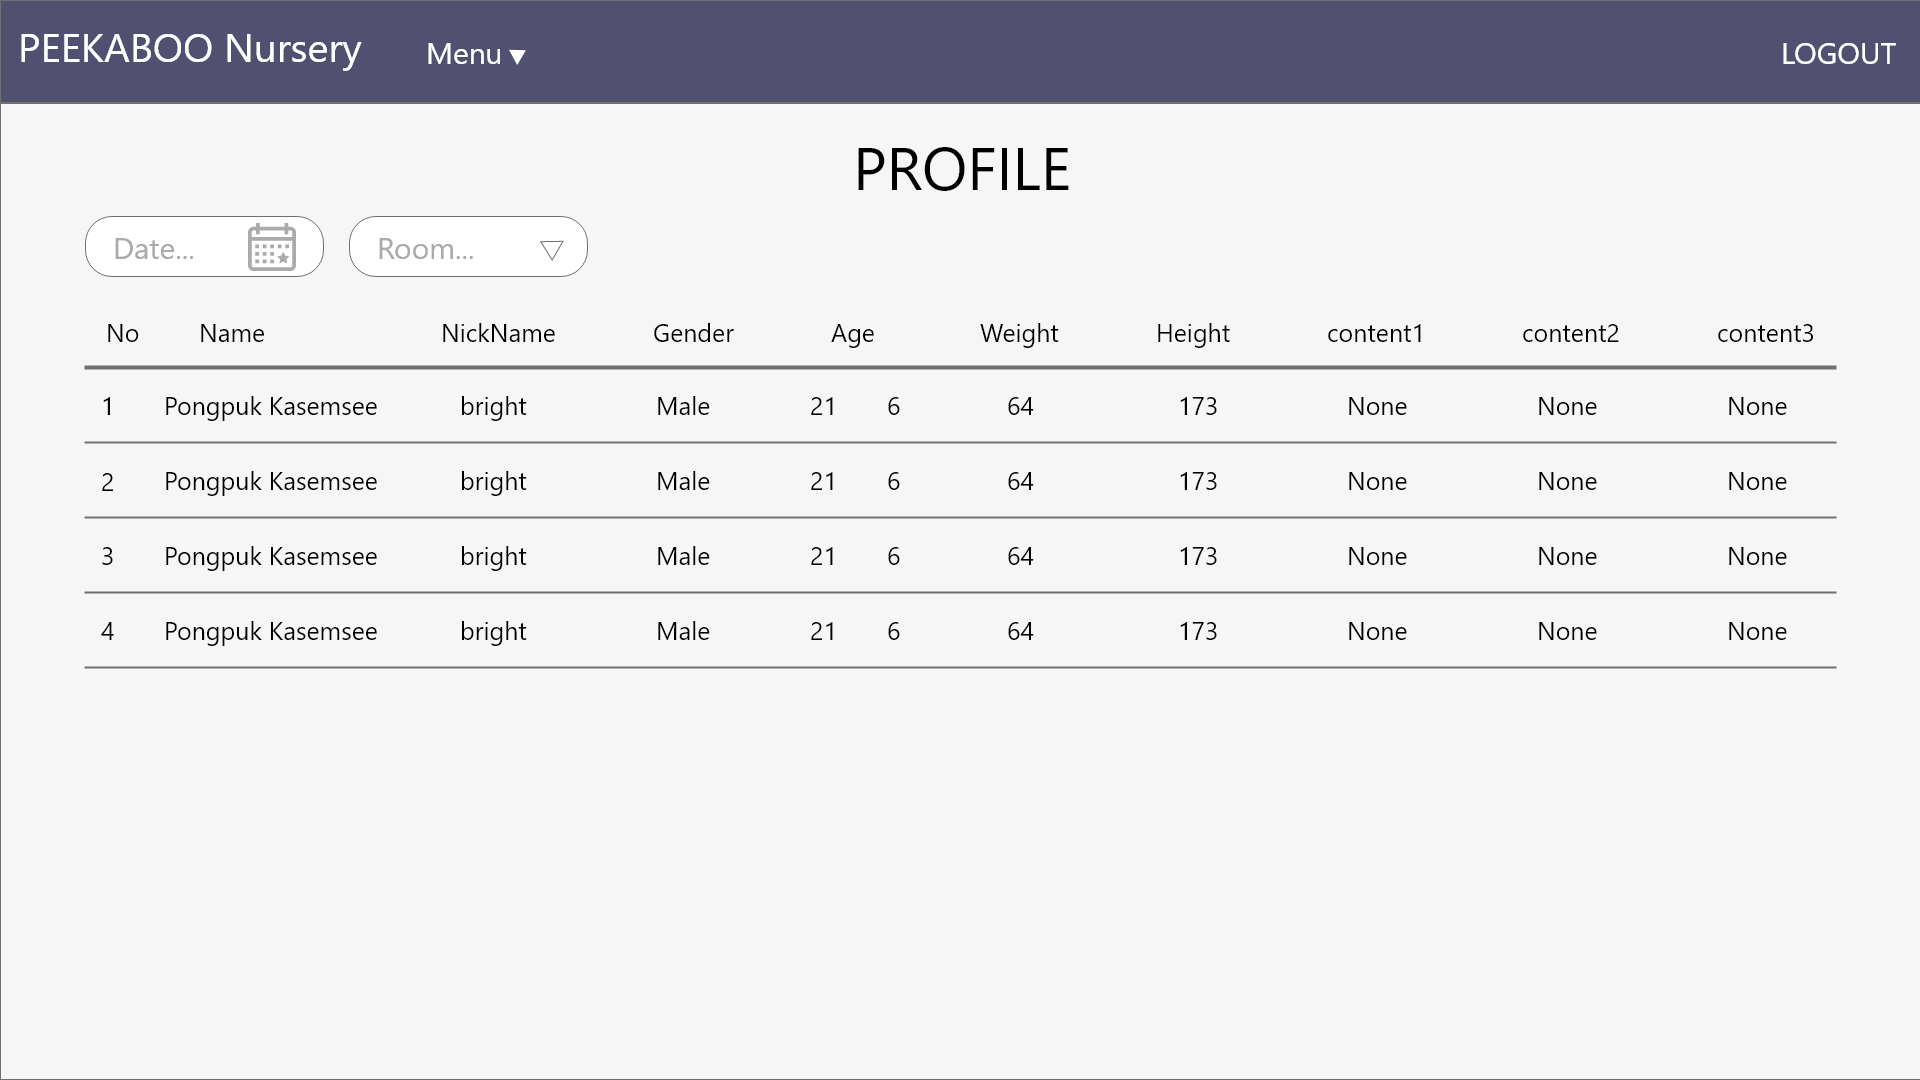
\includegraphics[width=\linewidth]{images/ProfileOnePage.png}
  \end{center}
  \caption[Poem]{Profile Page}
  \label{fig:Profile}
  \end{figure}

\begin{figure}
  \begin{center}
  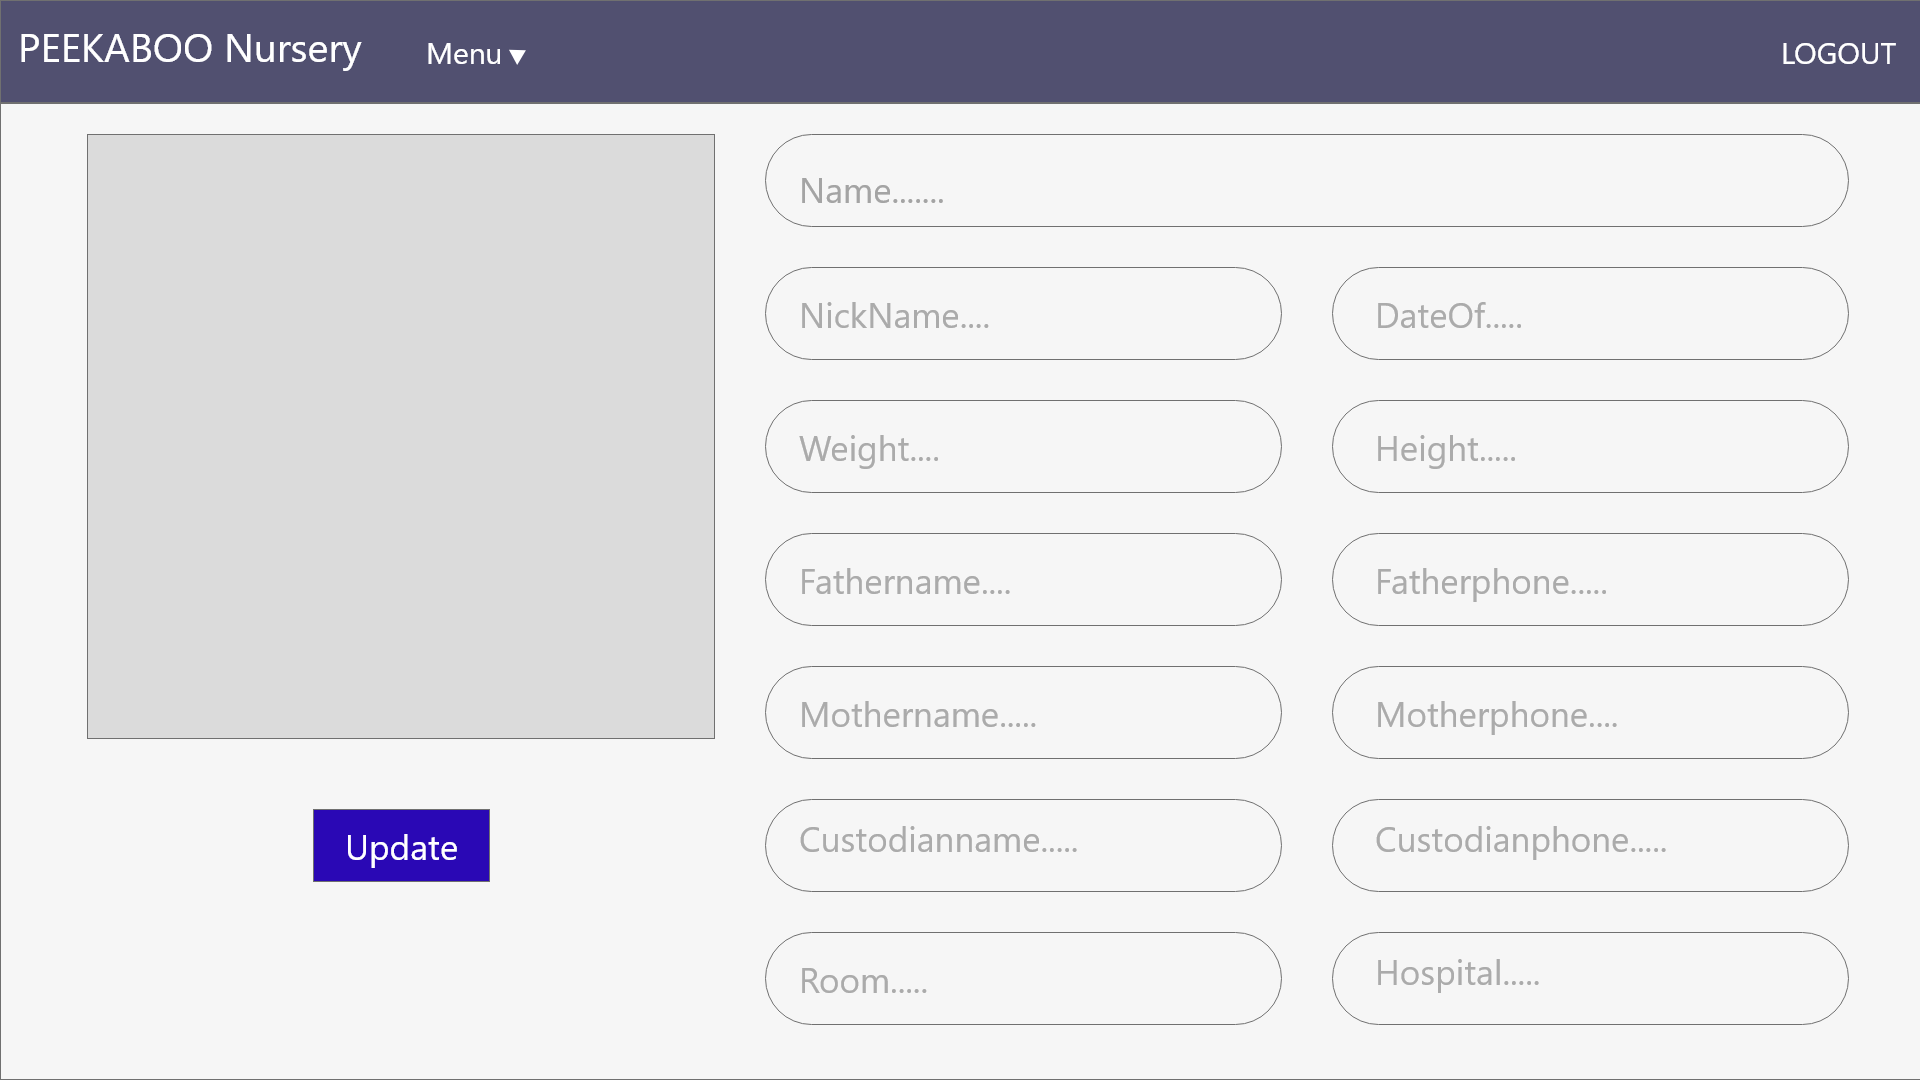
\includegraphics[width=\linewidth]{images/ProfileTwoPage.png}
  \end{center}
  \caption[Poem]{Profile Page}
  \label{fig:ProfileTwo}
  \end{figure}

\begin{figure}
  \begin{center}
  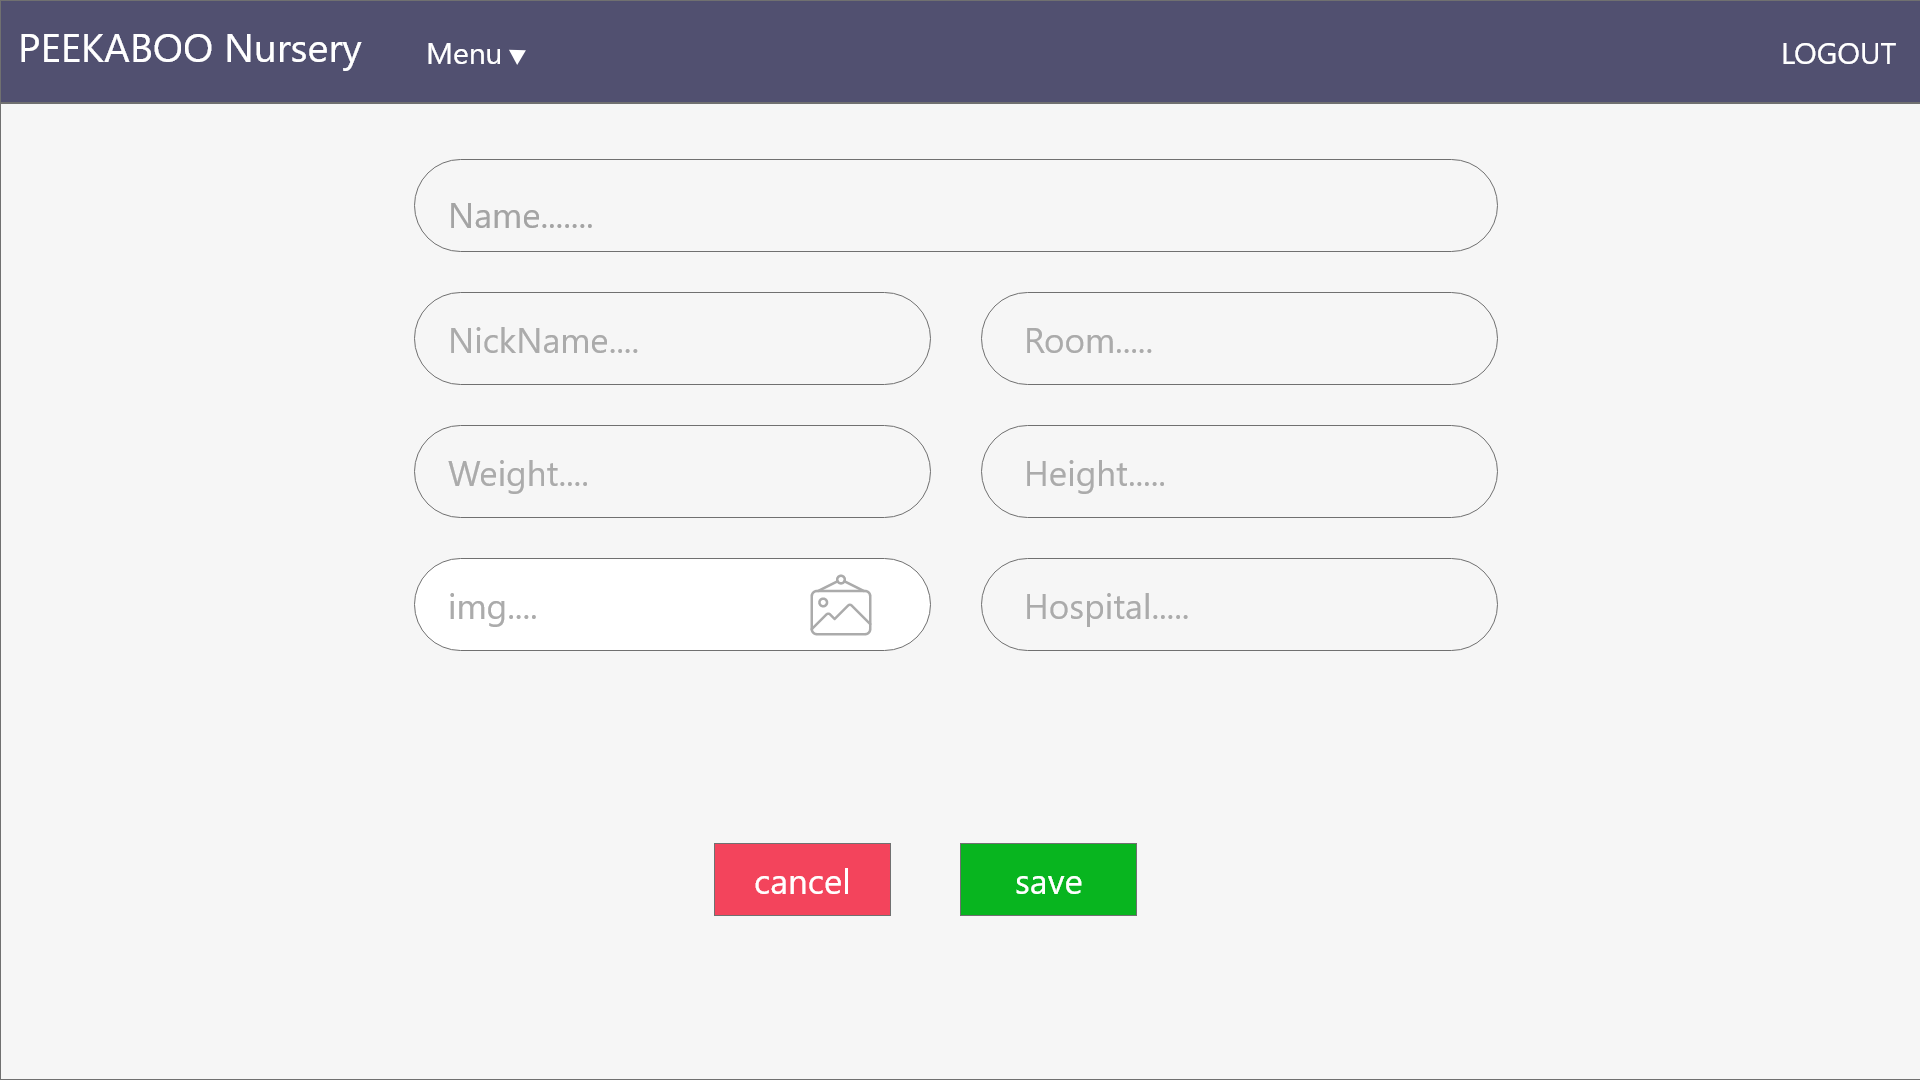
\includegraphics[width=\linewidth]{images/updateprofilePage.png}
  \end{center}
  \caption[Poem]{Update Profile Page}
  \label{fig:UpdateProfile}
  \end{figure}

\begin{figure}
  \begin{center}
  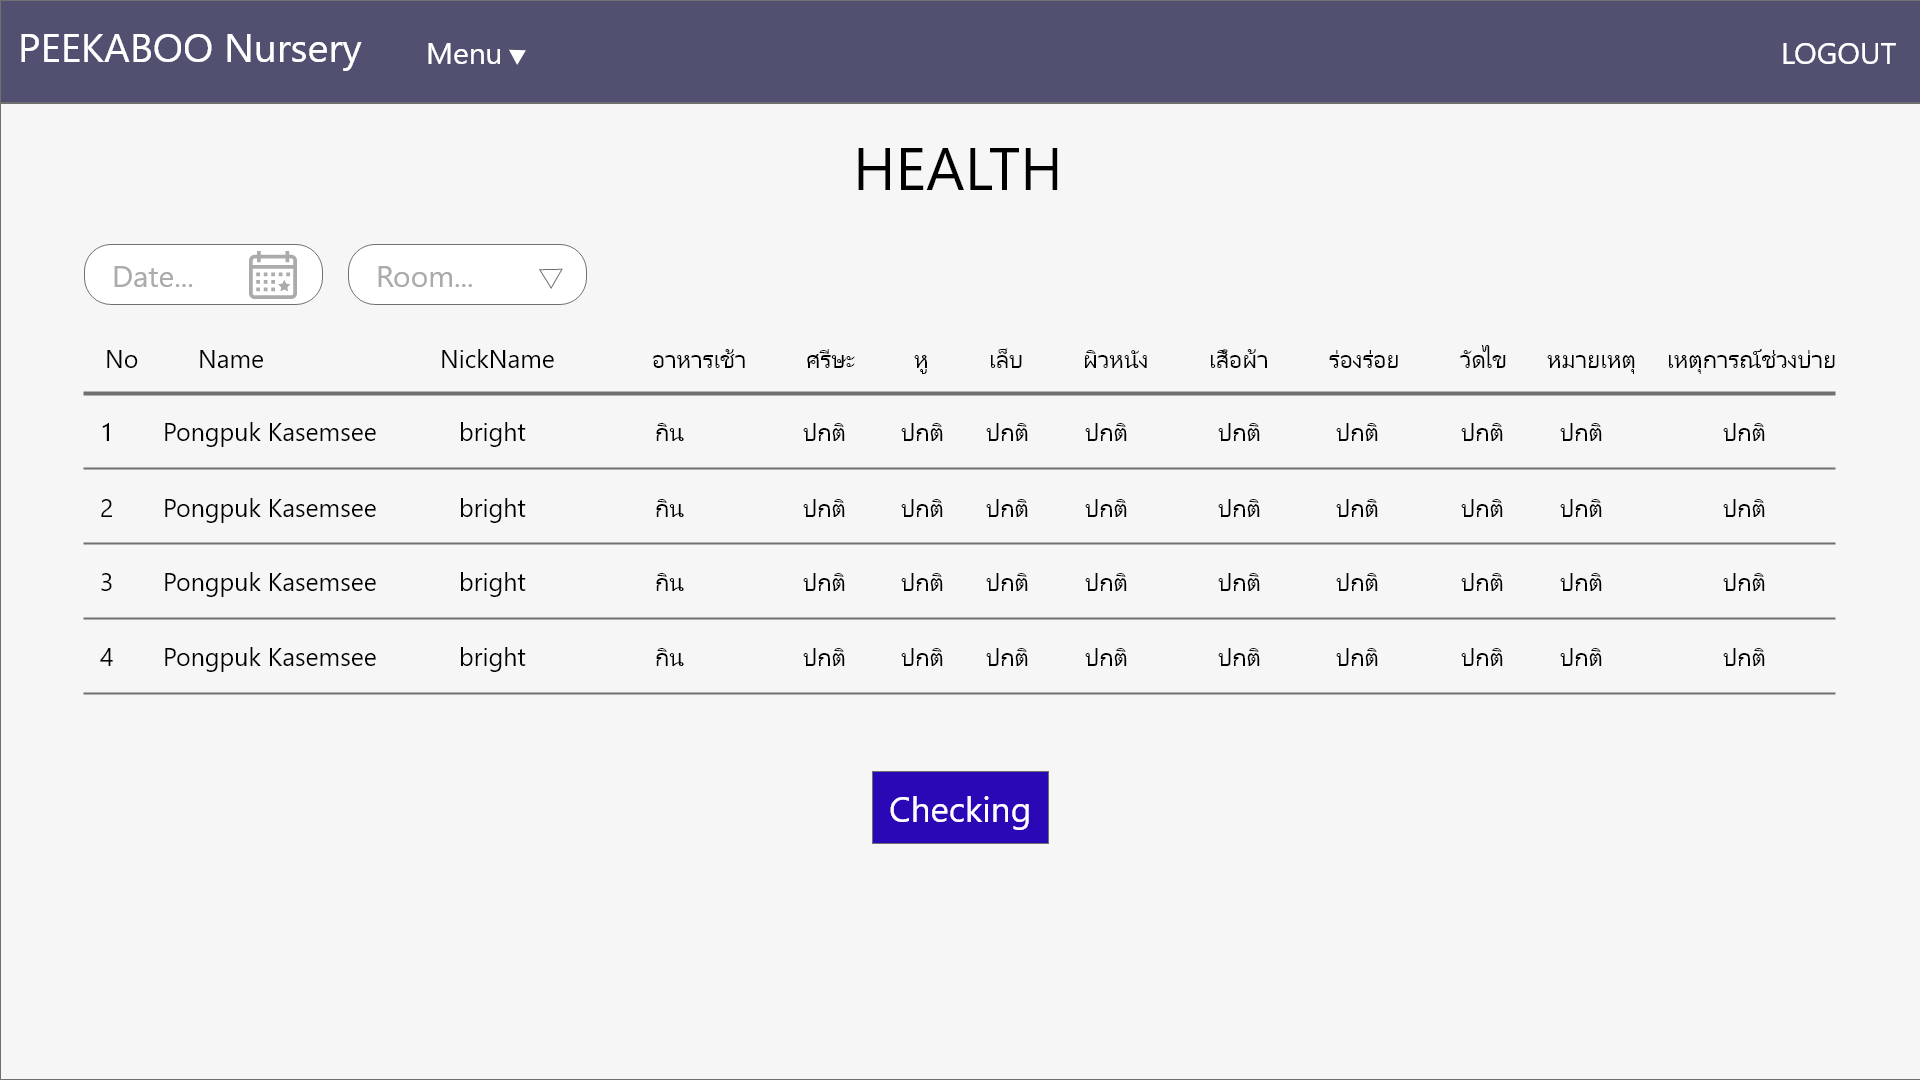
\includegraphics[width=\linewidth]{images/HealthPage.png}
  \end{center}
  \caption[Poem]{Health Page}
  \label{fig:Health}
  \end{figure}

\begin{figure}
  \begin{center}
  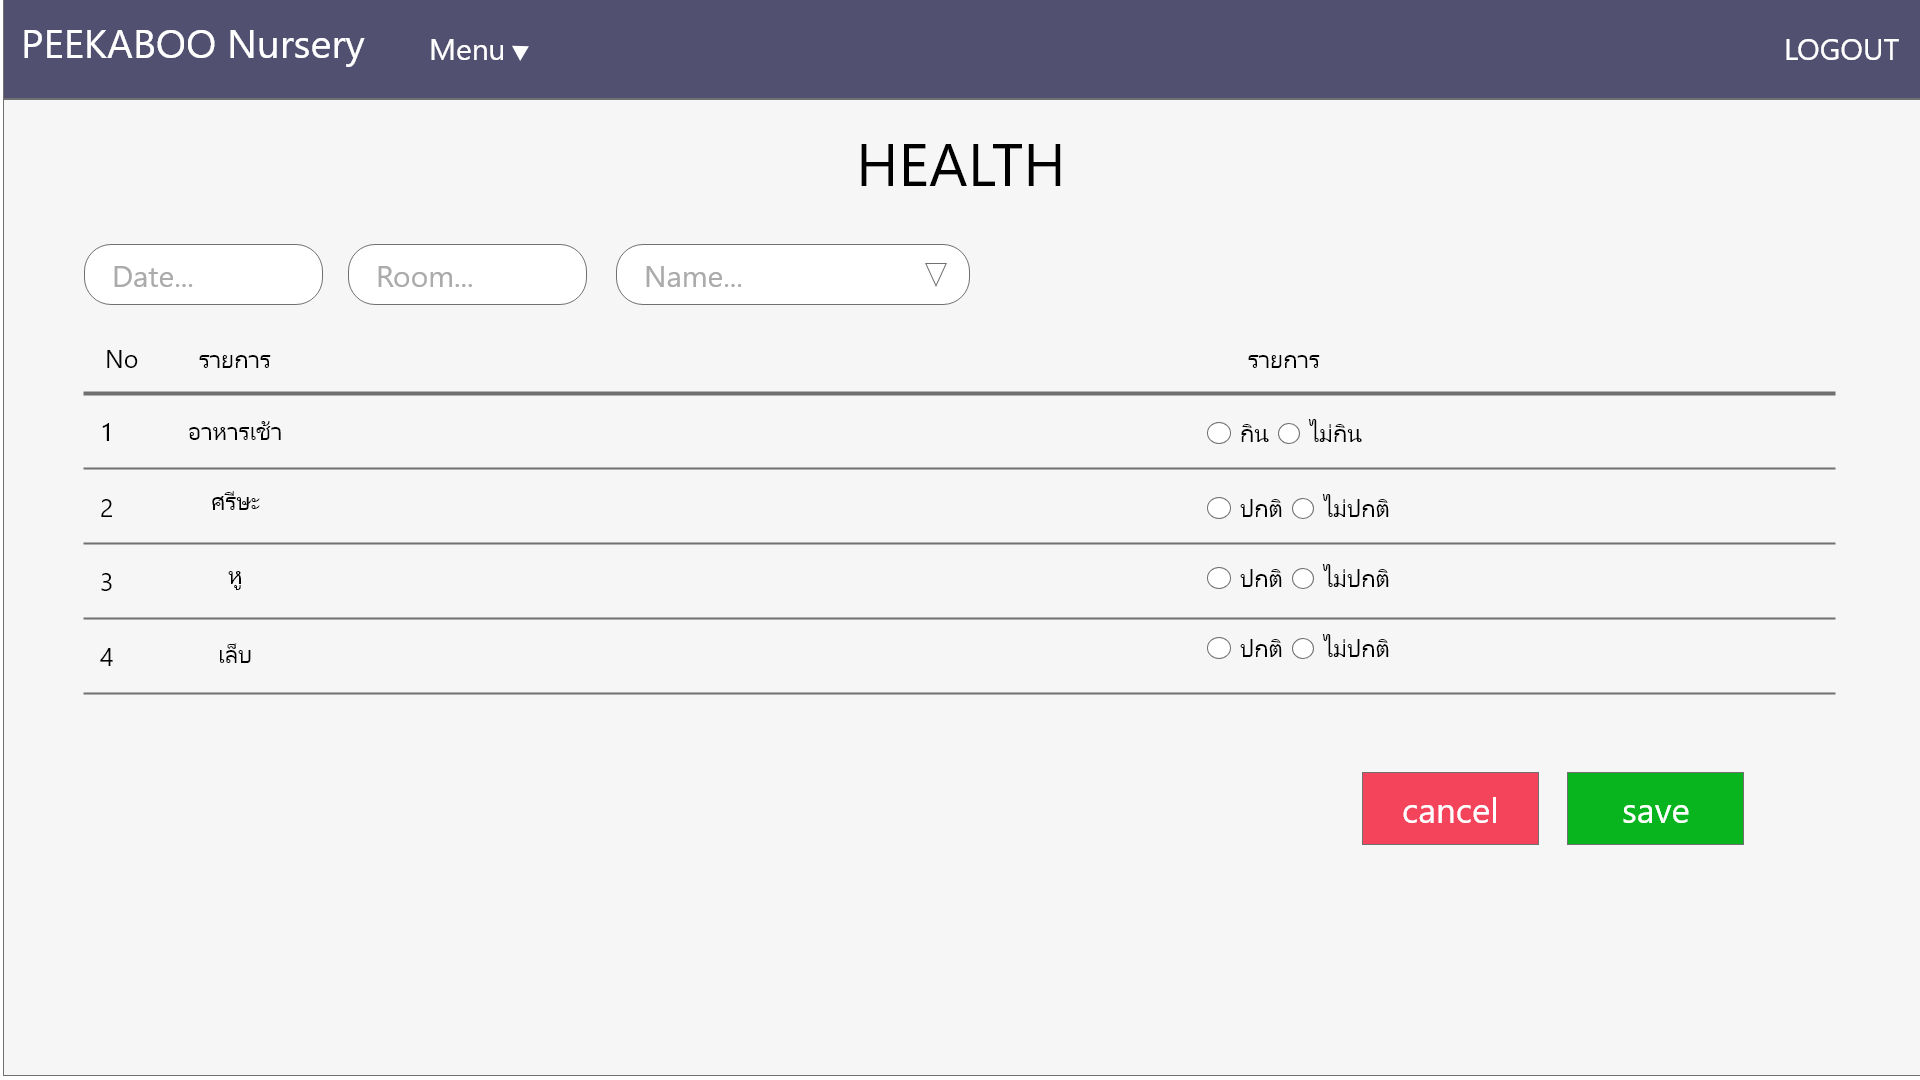
\includegraphics[width=\linewidth]{images/HealthPageChecking.png}
  \end{center}
  \caption[Poem]{Health Checking Page}
  \label{fig:CheckHealth}
  \end{figure}

\begin{figure}
  \begin{center}
  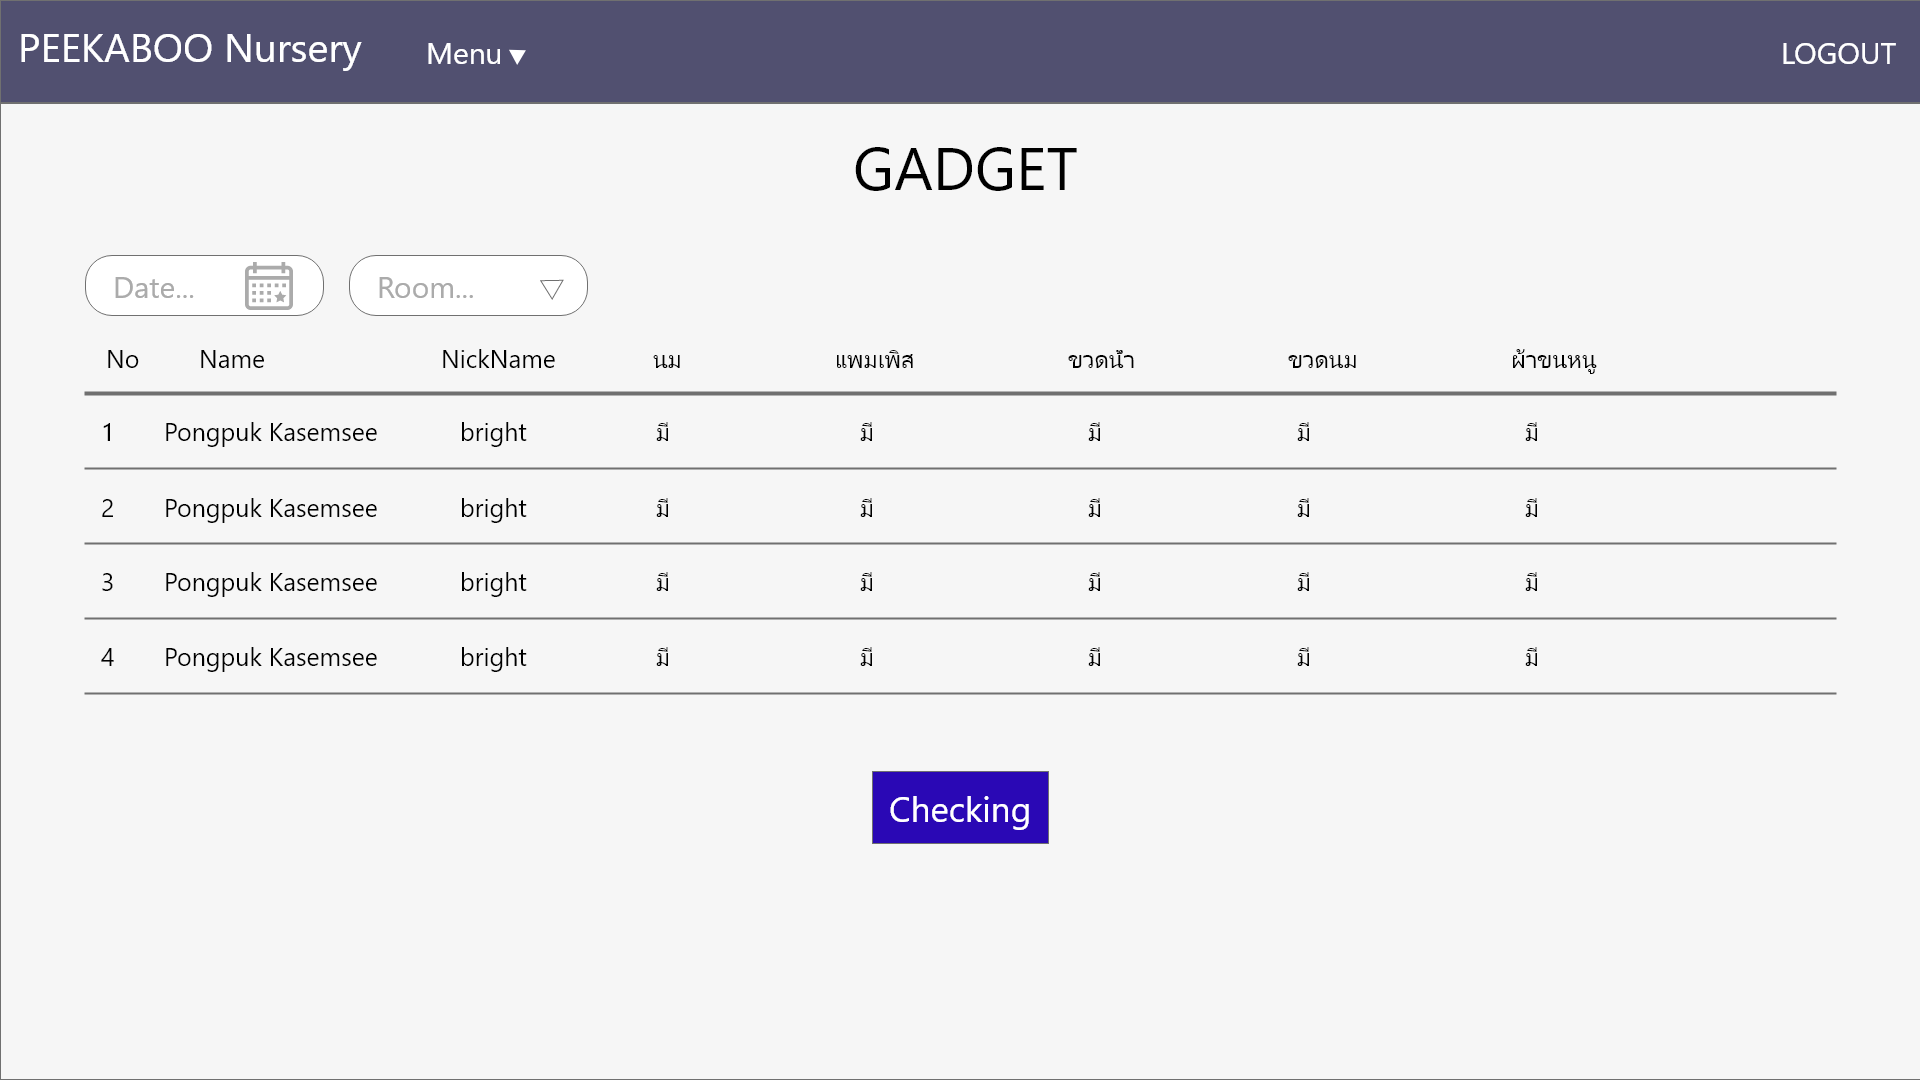
\includegraphics[width=\linewidth]{images/gadgetPage.png}
  \end{center}
  \caption[Poem]{gadget Page}
  \label{fig:Gadget}
  \end{figure}

\begin{figure}
  \begin{center}
  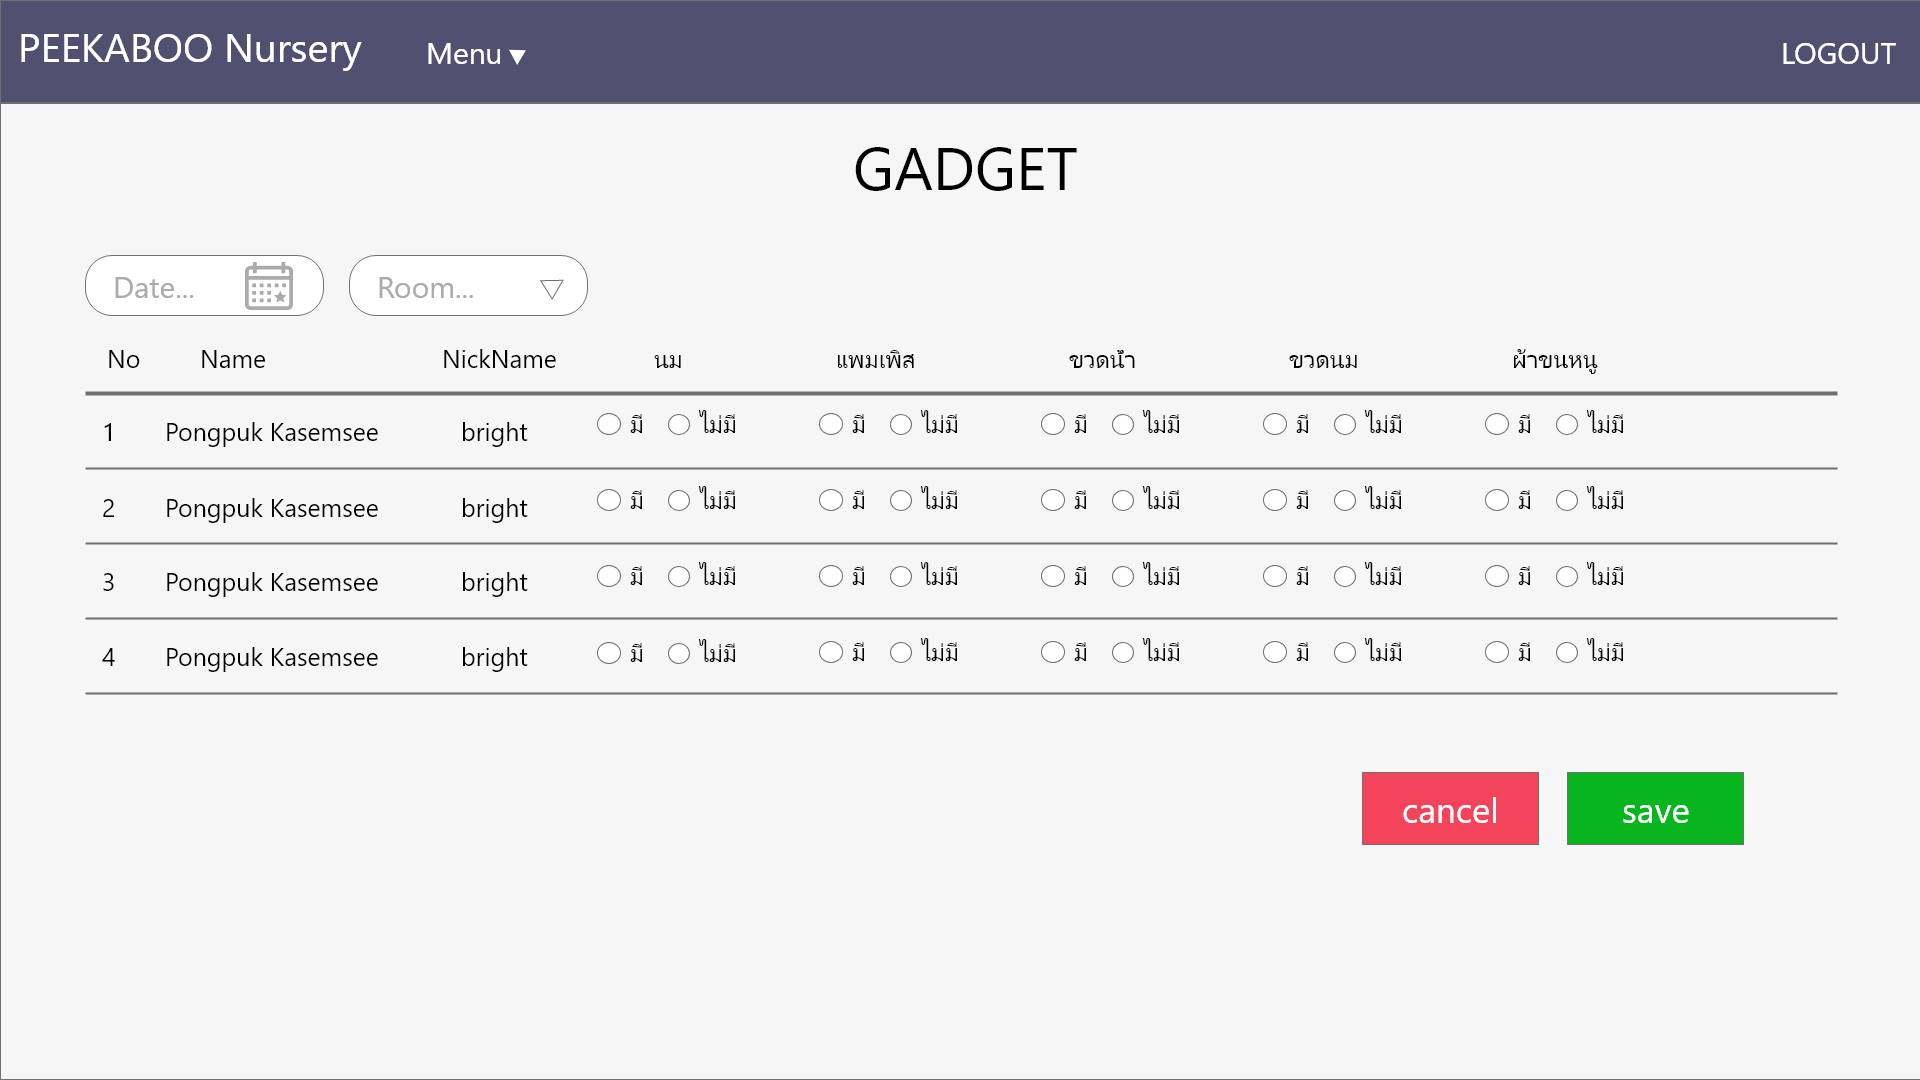
\includegraphics[width=\linewidth]{images/gadgetPageChecking.png}
  \end{center}
  \caption[Poem]{Gadget Checking Page}
  \label{fig:CheckGadget}
  \end{figure}

\begin{figure}
  \begin{center}
  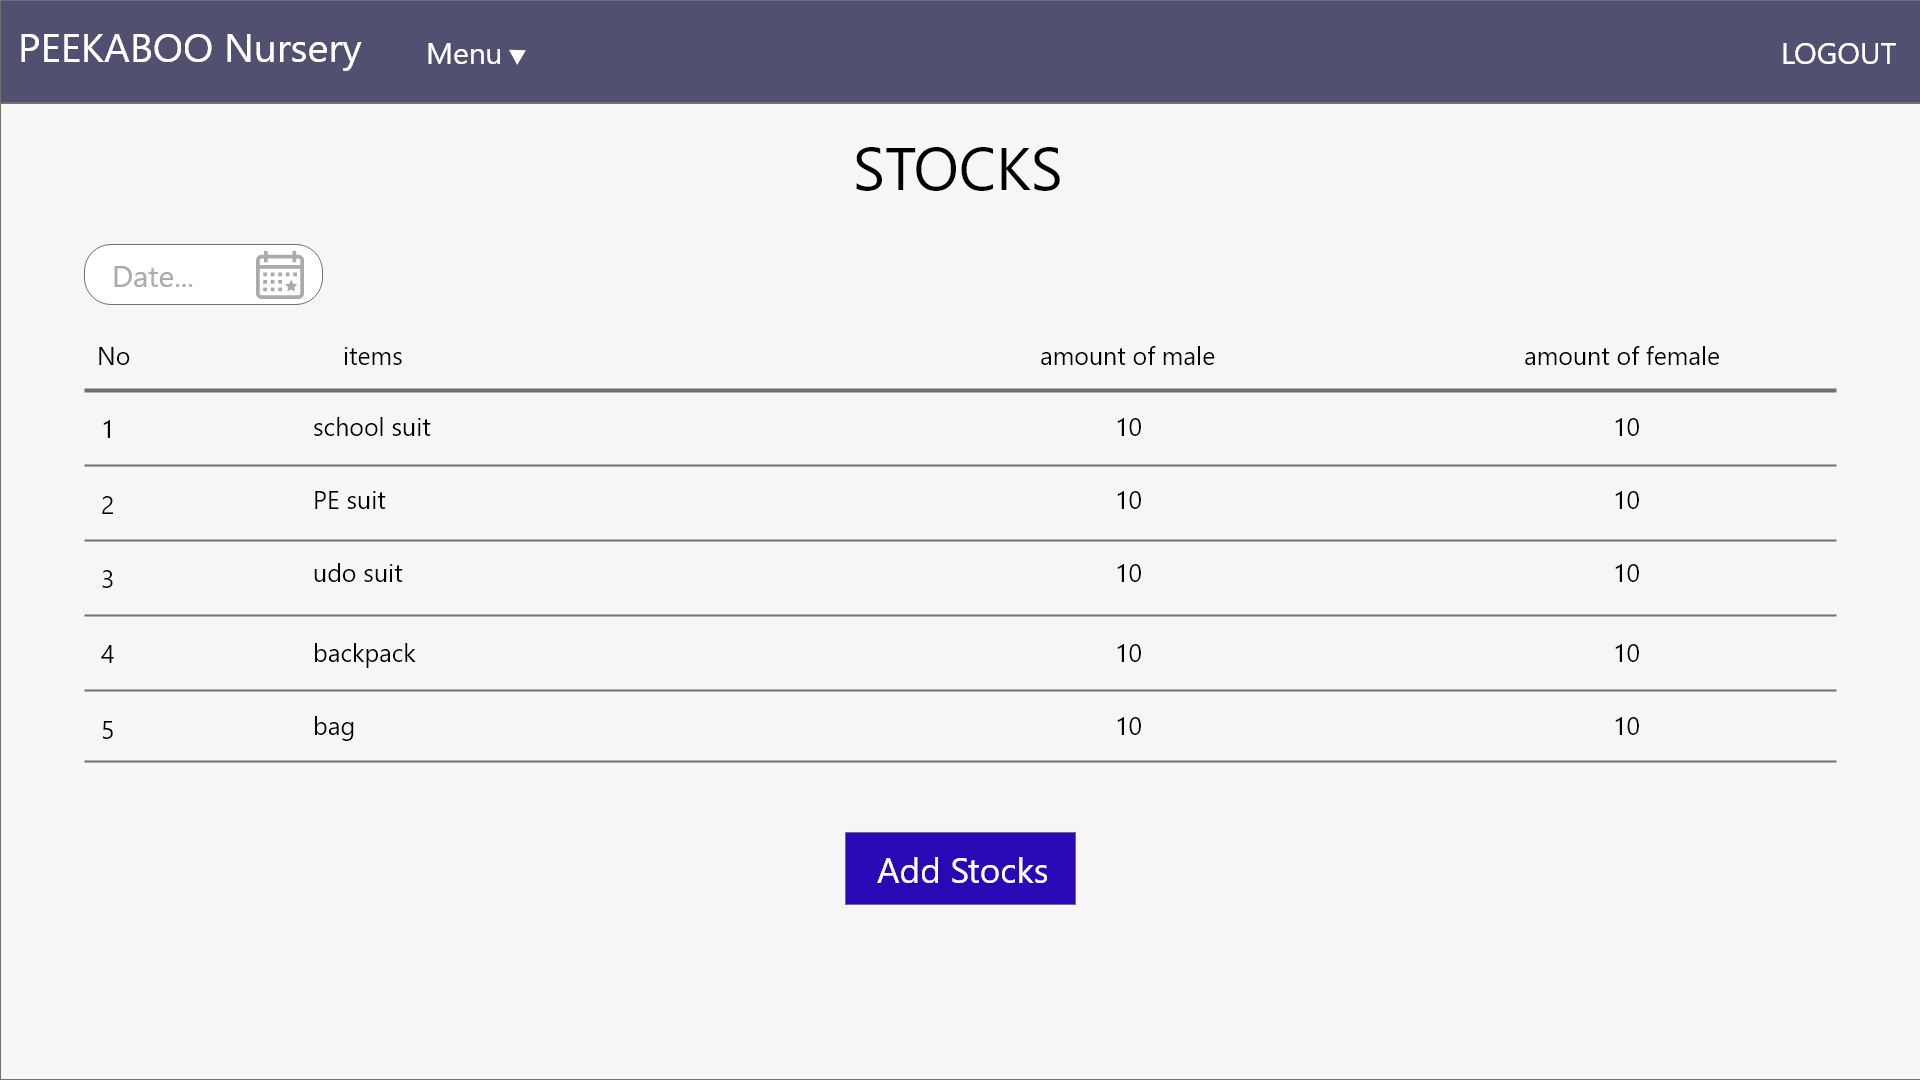
\includegraphics[width=\linewidth]{images/stockPage.png}
  \end{center}
  \caption[Poem]{Stock Page}
  \label{fig:Stock}
  \end{figure}

\begin{figure}
  \begin{center}
  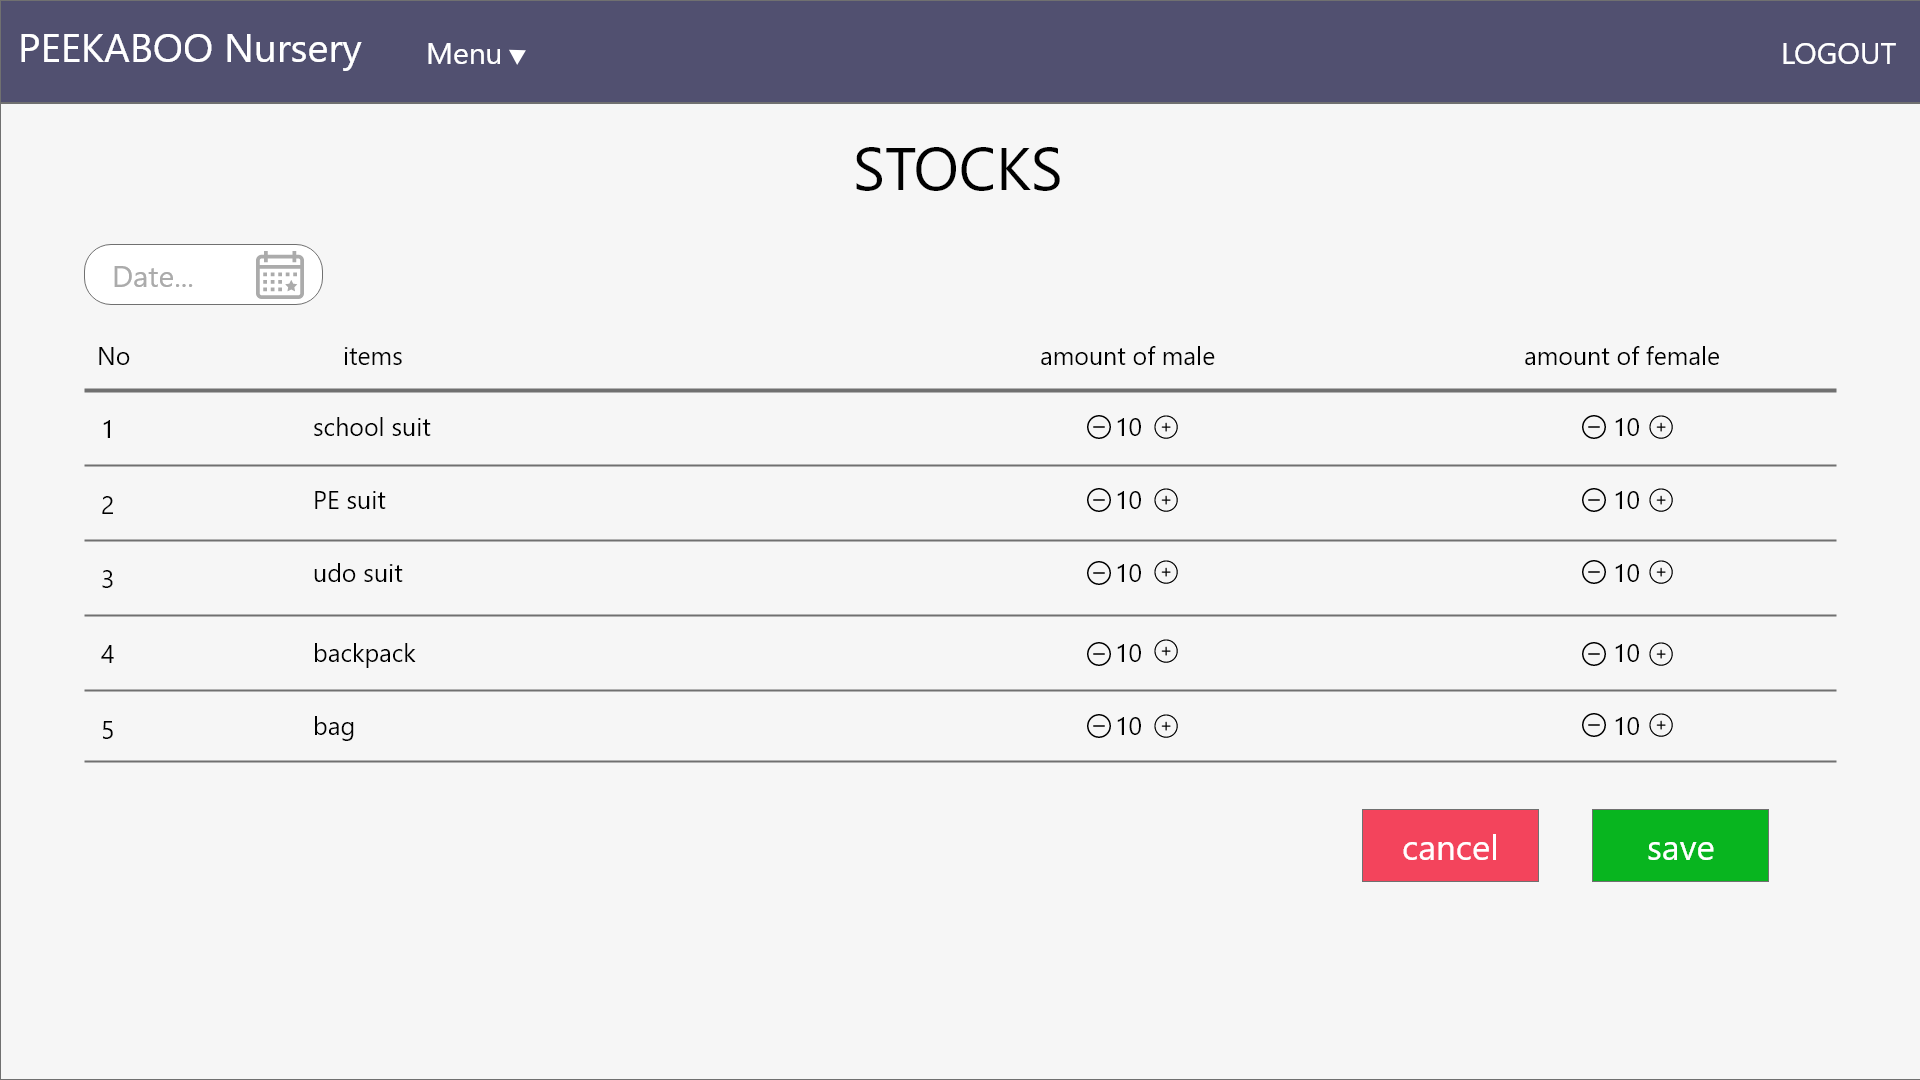
\includegraphics[width=\linewidth]{images/stockPageChecking.png}
  \end{center}
  \caption[Poem]{Stock Checking Page}
  \label{fig:CheckStock}
  \end{figure}

\begin{figure}
  \begin{center}
  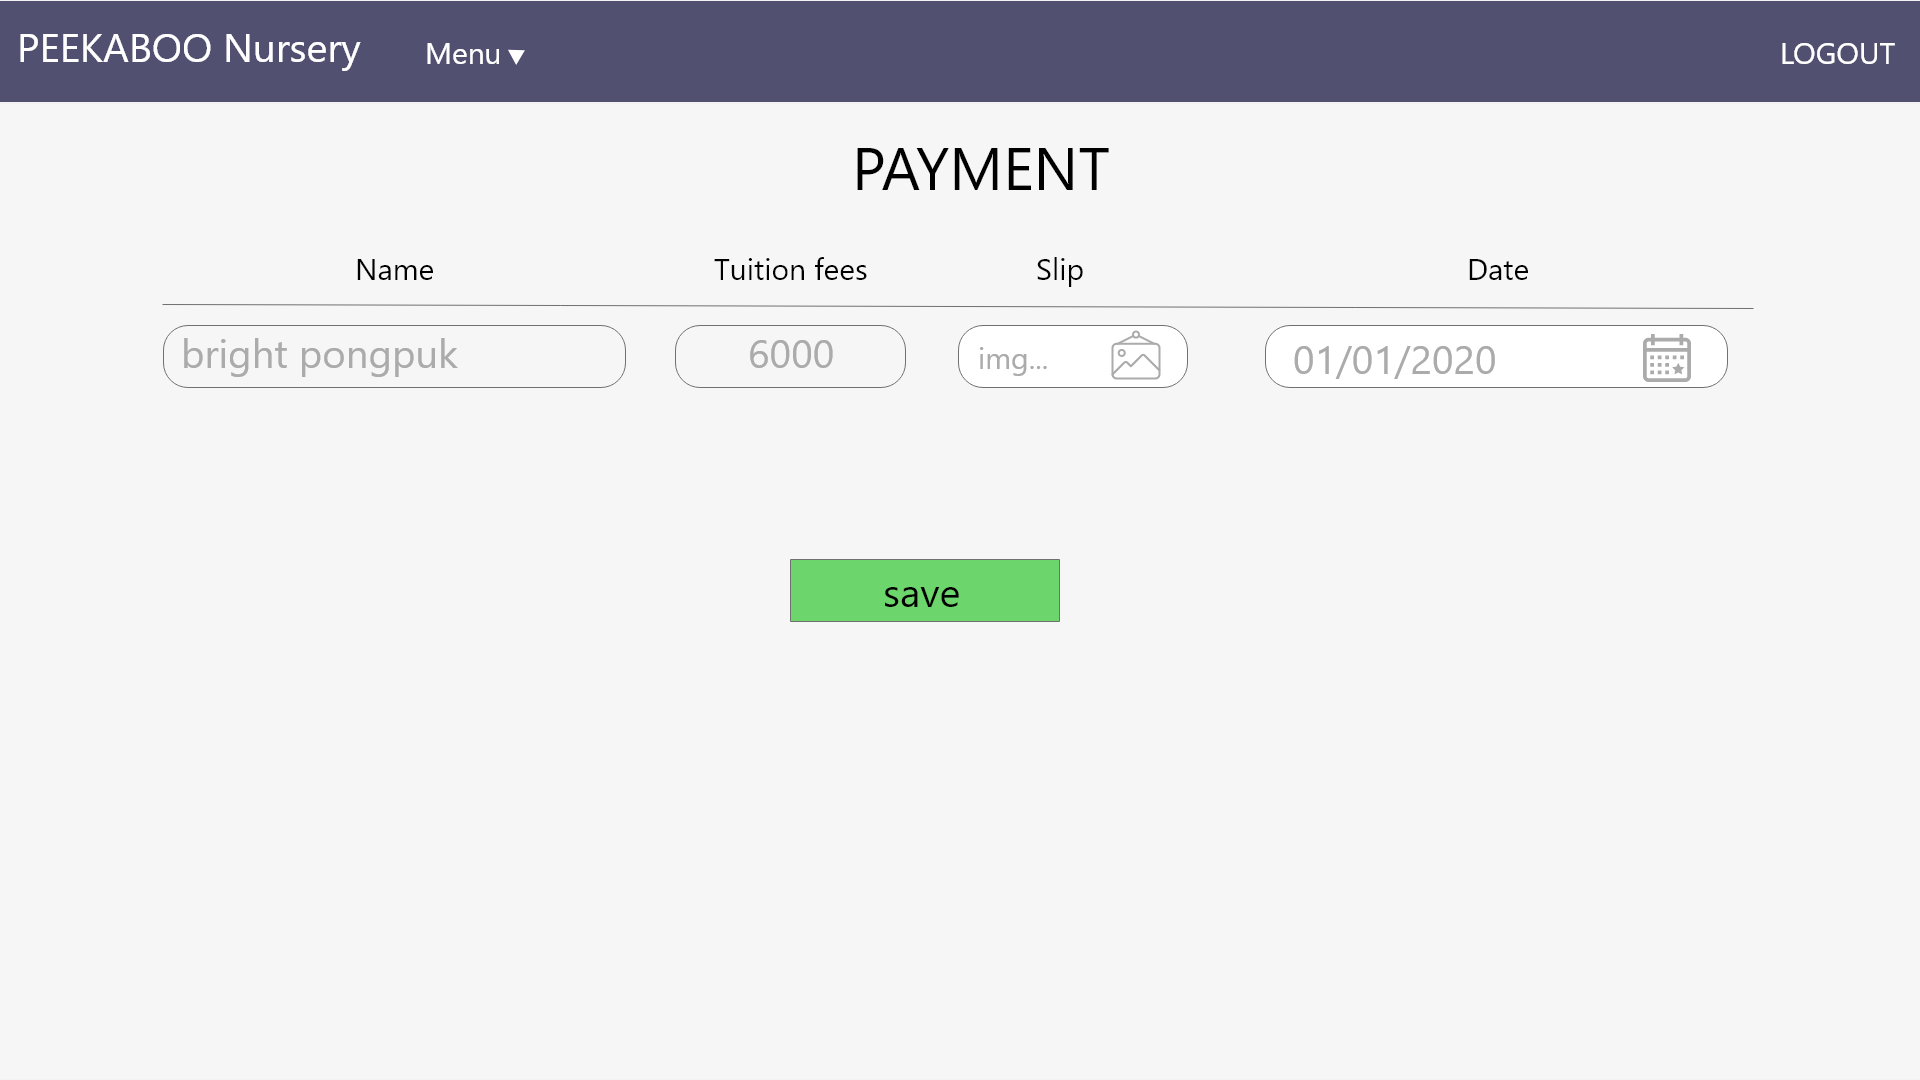
\includegraphics[width=\linewidth]{images/paymentPage.png}
  \end{center}
  \caption[Poem]{Payment Page}
  \label{fig:Payment}
  \end{figure}
\begin{enumerate}
  \item RegisterPage คือ หน้าแบบฟอร์มในการลงทะเบียนเด็กในการเข้าเรียน Nursery รูปที่~\ref{fig:register}
  \item  ProfilePage คือ หน้าที่ใช้ในการจัดการกับประวัติส่วนตัวของเด็ก สามารถแสดงข้อมูลและแก้ไขข้อมูลของเด็กแต่ละคนได้ รูปที่~\ref{fig:Profile} \ref{fig:ProfileTwo} \ref{fig:UpdateProfile}
  \item  Attendance คือ หน้าเช็คชื่อเด็กรายวัน รูปที่~\ref{fig:Attendance} \ref{fig:CheckAttendance}
  \item  Health คือ หน้าเช็คสุขภาพเด็กรายวัน รูปที่~\ref{fig:Health} \ref{fig:CheckHealth}
  \item  Gadget คือ หน้าเช็คของเด็กรายวัน รูปที่~\ref{fig:Gadget} \ref{fig:CheckGadget}
  \item  Stock คือ หน้าจัดการของใช้สำหรับเด็กทั้งหมดใน Nursery รูปที่~\ref{fig:Stock} \ref{fig:CheckStock}
  \item  Payment คือ หน้าที่ใช้จัดการกับใบเสร็จ  ประวัติการจ่ายเงินค่าเล่าเรียน รูปที่~\ref{fig:Payment}
\end{enumerate}








\subsection{Architecture}

ระบบหลักๆที่ทางผู้พัฒนาใช้จะเป็นระบบแบบ Client-Server คือในทางฝั่ง Client จะใช้ React ในการพัฒนาแบบ Web-browser ให้ทางผู้ใช้ส่ง Requests มายังฝั่ง Server เพื่อที่จะทำงานต้องที่ผู้ใช้ต้องการ ซึ่งฝั่ง Server 
จะพัฒนาโดย Express.js ทางฝั่งนี้ก็จะ query ข้อมูลจากทางฐานข้อมูลที่เก็บไว้บน Mongodb Atlas เมื่อได้รับข้อมูลแล้วก็จะทำการส่ง Responses กลับไปยัง Client เพื่อให้ผู้ใช้สามารถทำงานในส่วนที่ต้องการได้ตามที่ต้องการ

\section{ขั้นตอนการดำเนินงาน}
\subsection{Discovery}
\begin{itemize}
  \item สำรวจและสอบถามปัญหาจากstakeholder
  \item นำปัญหาต่างหรือrequirementsมาวิเคราะห์
  \item สรุปผลแล้วนำrequirementsที่ได้จากการวิเคราะห์ไป  ทำต่อในขั้นตอนถัดไป
\end{itemize}

\subsection{Design}
\begin{itemize}
  \item ออกแบบหน้า UI/UX โดย Adobe XD
  \item ออกแบบฐานข้อมูลโดย Draw.io
  \item ออกแบบ
\end{itemize}

\subsection{Develop}
\begin{itemize}
  \item สร้าง Database
  \item เขียน Backend ตามที่ได้ Design มาในขั้นตอนก่อนหน้า
  \item เขียน Frontend แล้วทดสอบยิง Api ไปยังฝั่ง Backend
  \item เชื่อมโค้ด Frontend กับ Backend ผ่าน Api
\end{itemize}

\subsection{Testing}
